\section{Introduction}

Data centers are responsible for driving large-scale web applications such as web search, storage, advertising, and social network composition ~\cite{chen_understanding_2009, alizadeh_data_2010}. These applications generate diverse communcation patterns with strict throughput and latency requirements. In particular, many distributed web applications rely on a workflow patterns in which requests are broken down and distributed to multiple workers, which perform tasks simultaneously and return responses to an aggregator ~\cite{chen_understanding_2009, alizadeh_data_2010}. As a result, data centers need to support bursts of many-to-one traffic traversing shared bottlenecks without affecting the throughput of long-lived flows needed to update and maintain application data ~\cite{alizadeh_data_2010}.

In order to accomodate the workload generated by these applications while maintaining cost efficiency, modern data centers typically feature high speed links with very low propogation delays, connecting nodes via low-cost switches with shallow buffers ~\cite{chen_understanding_2009, hamilton_designing_2007, alizadeh_data_2010}. The majority of communication between nodes is over TCP, which was designed based on the characteristics of wide area networks, where roundtrip times (RTTs) are orders of magnitude greater than in data centers ~\cite{chen_understanding_2009}. As a result, while traditional TCP congestion control mechanisms which are usually considered ``good enough'' in the context of the internet, TCP does not perform well when faced with traffic patterns typical of data center networks ~\cite{chen_understanding_2009, phanishayee_measurement_2008}. 

In particular, the traffic patterns common to data center networks suffer a number of impairments due to problems with traditional TCP congestion control mechanisms. In the synchronized many-to-one scenarios common to distributed applications such as MapReduce, TCP connections experience throughput collapse, or incast congestion. In this scenario, goodput at the receiver drops dramatically as simultaneous TCP flows from synchronized senders floods the buffer of a bottleneck switch, causing packet loss and large queueing delays ~\cite{chen_understanding_2009, phanishayee_measurement_2008, dean_mapreduce:_2004}.

In addition, long lived background flows tend to keep switch buffers full, leading to increased queueing delays for latency sensitive traffic. Moreover, improving resource utilization through dynamic buffer allocation means that long lived flows can even cause buffer pressure that impacts flows traversing other ports on a switch ~\cite{alizadeh_data_2010}. More generally, TCP's loss based congestion control mechanism means that large switch buffers are kept full, which means that traffic is subject to large queueing delays even in the absence of packet loss, while packet loss at switches with small buffers is misinterpreted as network congestion leading to underutilization of network resources ~\cite{cardwell_bbr:_2016}.

This paper discusses a number of approaches to TCP congestion control aimed at improving the performance of TCP in data centers. In particular, Data Center TCP (DCTCP) is discussed in depth, and a number of key findings are reproduced using the Mininet network emulator.

\subsection{Data Center Traffic Patterns}

The applications running in modern data centers rely heavily on the \emph{partition/aggregate} design pattern, in which an application is broken in into hierarchical layers and time-sensitive requests at higher layers are divided and delegated to workers in the lower layers. Workers perform some component of a task and return a result to an aggregator, which is combined with results from other workers and passed back up through the hierarchy. 

\subsection{Impairments}

\subsubsection{Incast}

TCP throughput collapse, or TCP \emph{incast},  

\subsubsection{Queue Build-Up}

\subsubsection{Buffer Pressure}

\subsubsection{Buffer Bloat and Underflow}

\section{Improving TCP for Datacenters}

\subsection{Incast TCP}

\subsection{Multipath TCP}

\subsection{TCP BBR}

\subsection{Data Center TCP}

Data center TCP (DCTCP) attempts to address the problem of latency in partition/aggregate traffic by reducing queue length without affecting throughput for large TCP flows.

\section{Reproducing Key DCTCP Results}

\subsubsection{Methods}

Selected results from \cite{alizadeh_data_2010} were reproduced using the Mininet network emulator running on Ubuntu 12.04 with a patched version of the 3.2.18 Linux kernel patched to add in support for DCTCP. A custom utility was modified from the Mininet utilities repository to monitor queue length, and another utility was created to monitor bandwidth. 

\subsubsection{Results}

\begin{figure}
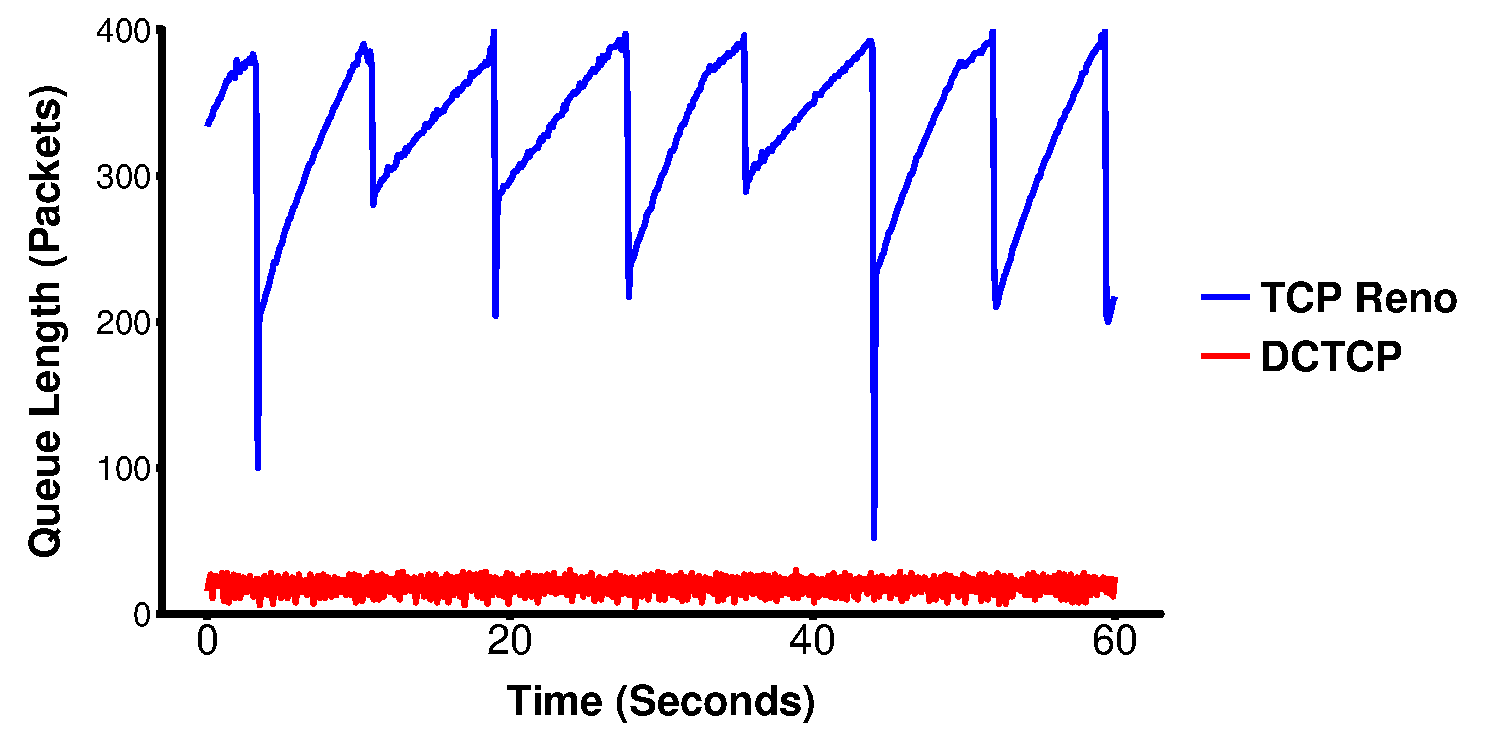
\includegraphics[height=1.75in,width=3.5in]{queue_2_flows}
\caption{Comparison of queue length over time between DCTCP and TCP Reno with 2 flows}
\end{figure}

\begin{figure}
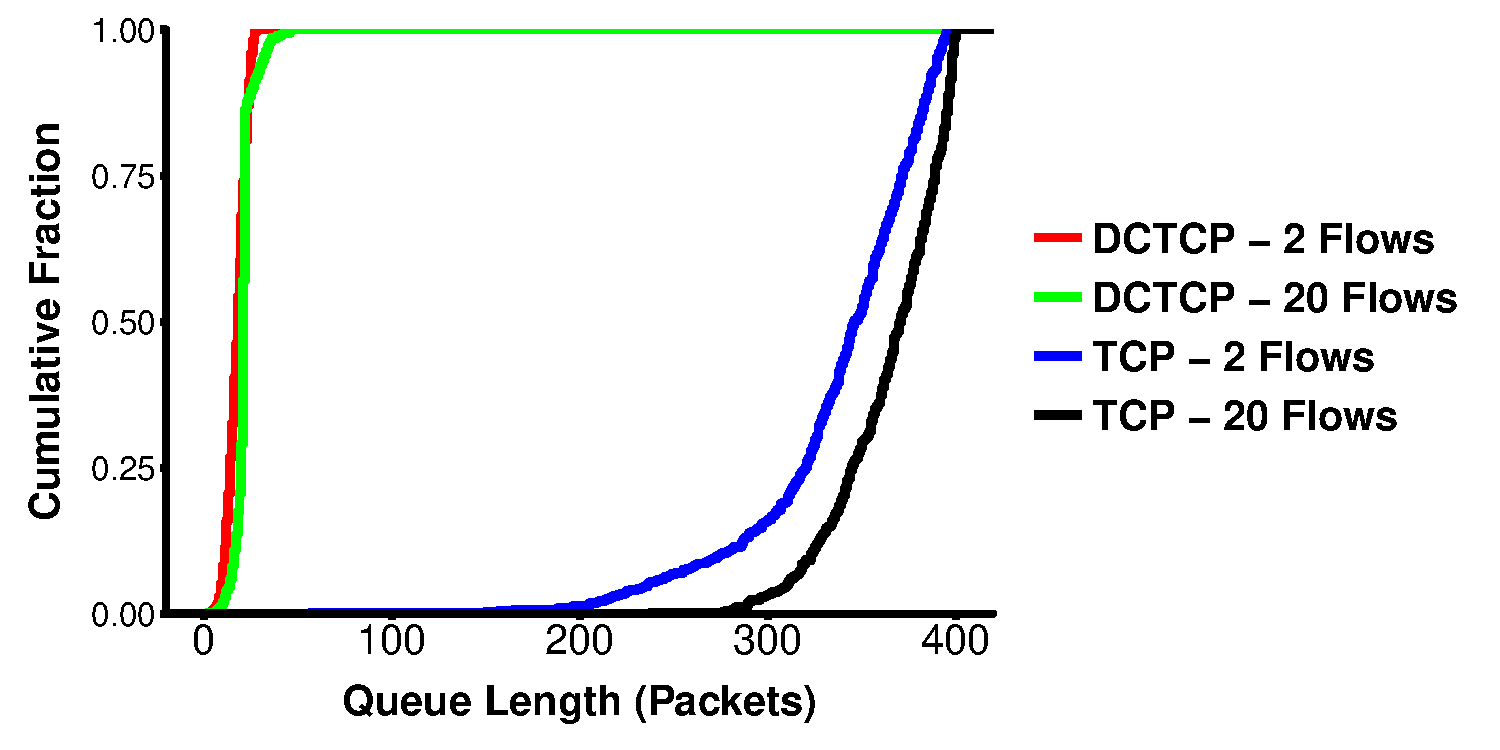
\includegraphics[height=1.75in,width=3.5in]{queue_cdf}
\caption{CDF of queue length for DCTCP and TCP Reno with 2 and 20 flows}
\end{figure}

\begin{figure}
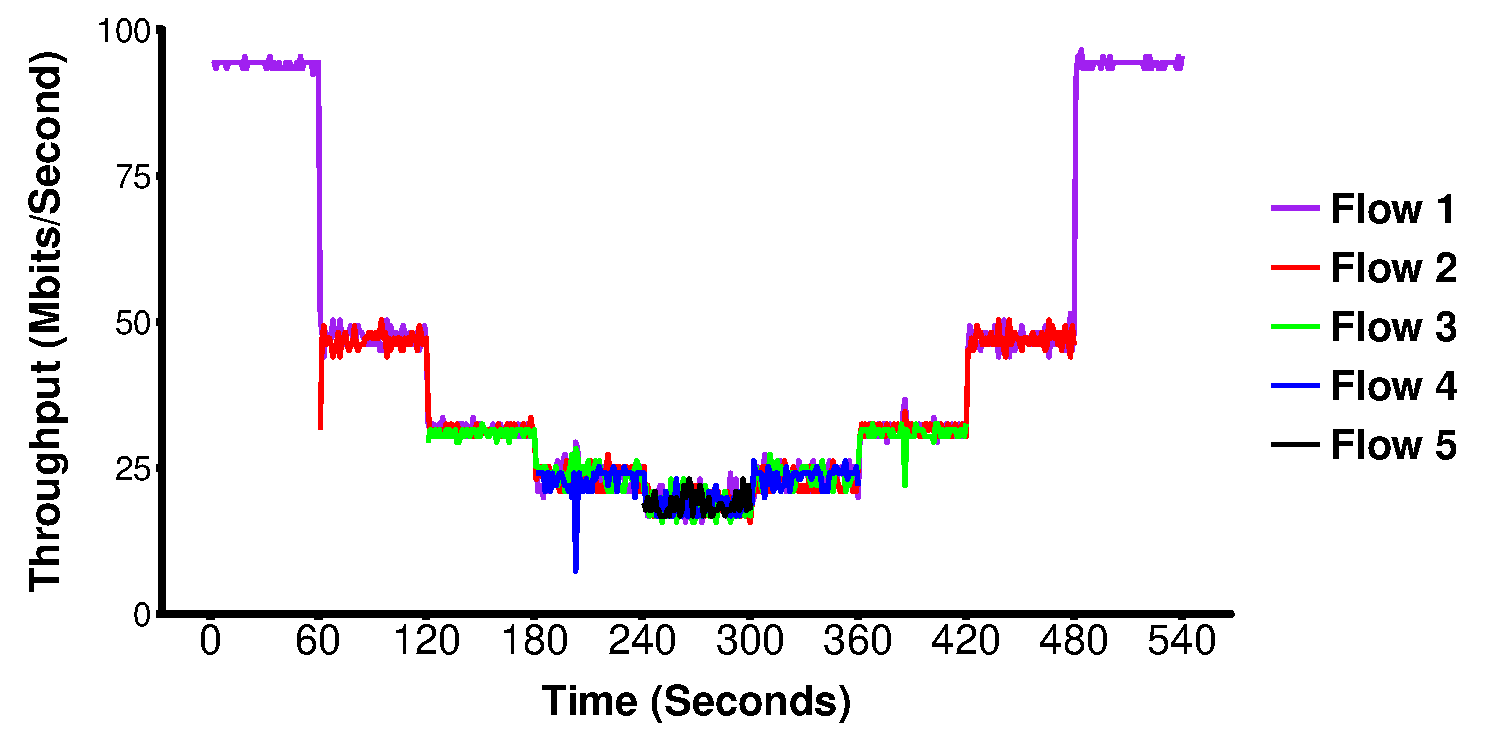
\includegraphics[height=1.75in,width=3.5in]{dctcp_converg}
\caption{Convergence of 5 flows DCTCP}
\end{figure}

\begin{figure}
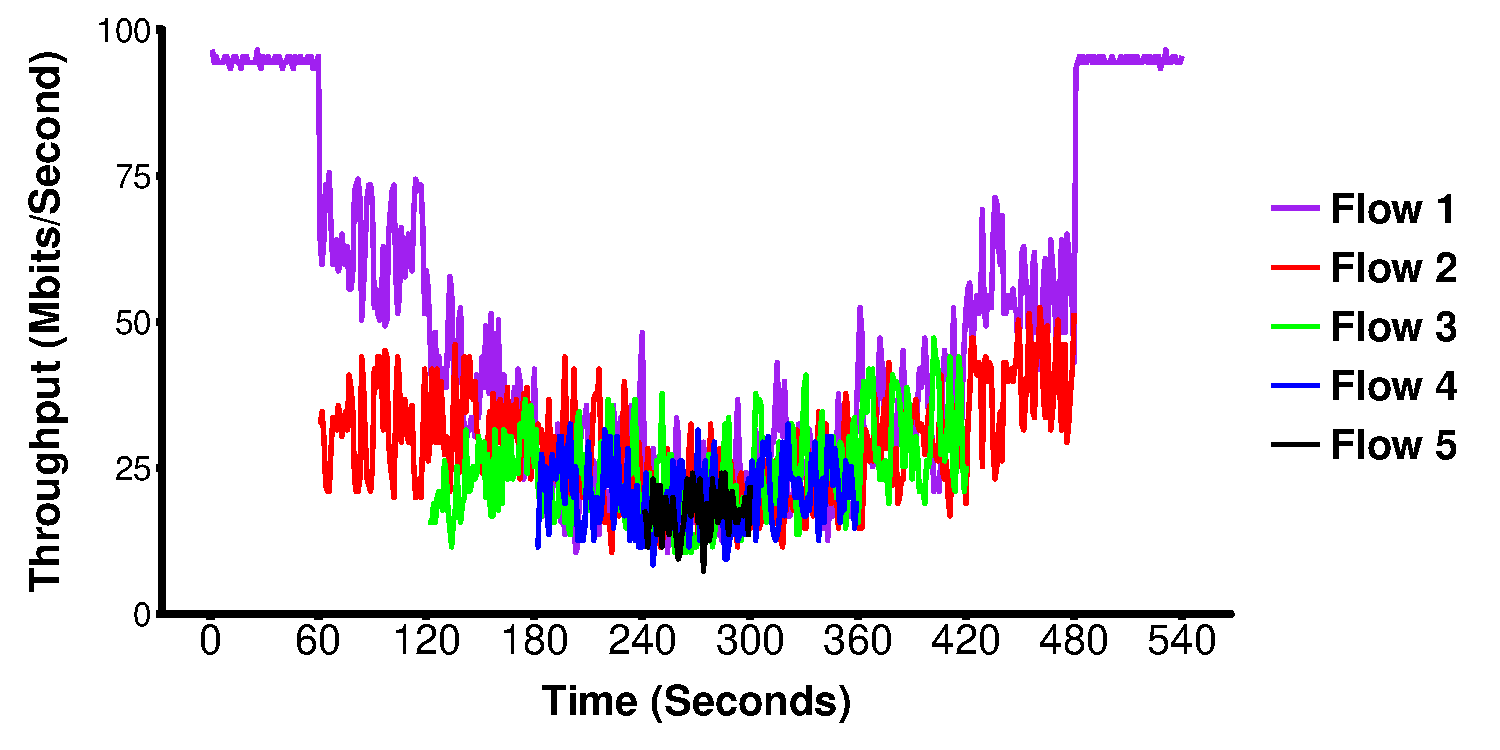
\includegraphics[height=1.75in,width=3.5in]{reno_converg}
\caption{Convergence of 5 flows TCP Reno}
\end{figure}

\begin{figure}
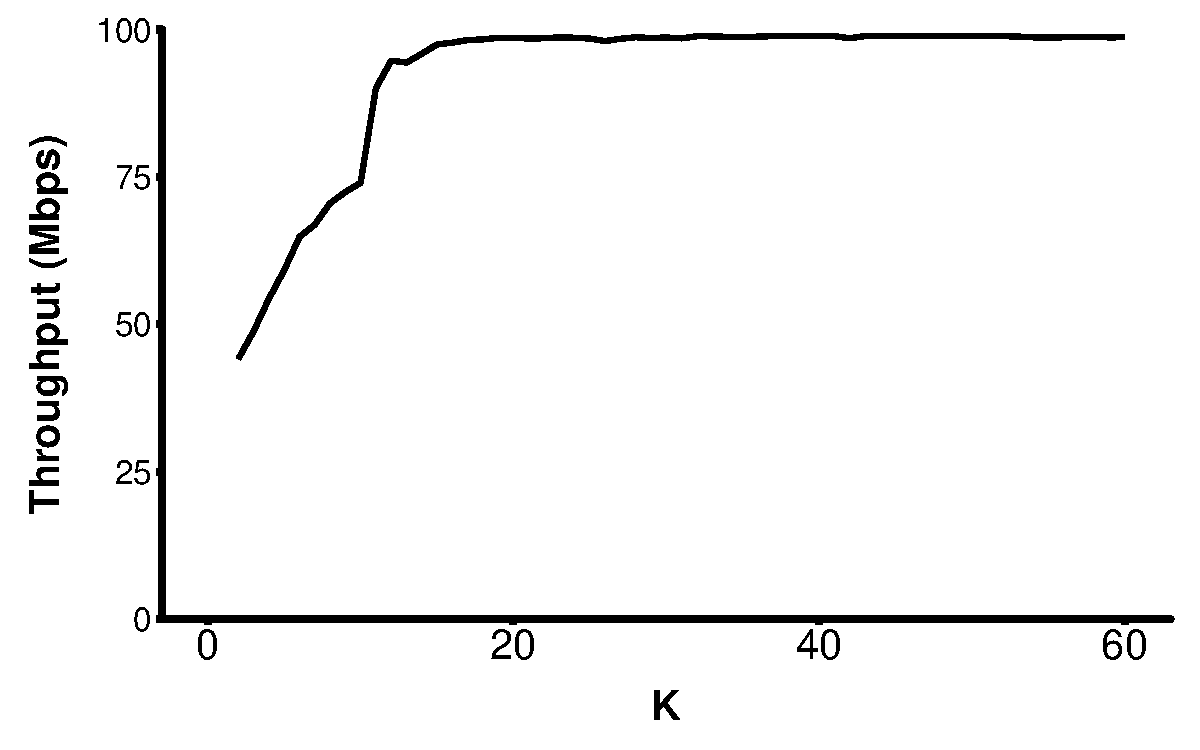
\includegraphics[height=2in,width=3in]{k_throughput}
\caption{DCTCP throughput for varying values of K}
\end{figure}

\subsubsection{Discussion}

\subsubsection{Limitations}

\section{Conclusions}

